\documentclass{standalone}

\usepackage{tikz}
\usepackage{tkz-euclide}
\usetikzlibrary{calc}
\usetikzlibrary{positioning}
\usetikzlibrary{arrows.meta}
\usetikzlibrary{shapes,snakes}

\usepackage{times}

\definecolor{myblue}{rgb}{0.0,0.5,0.8}

\begin{document}
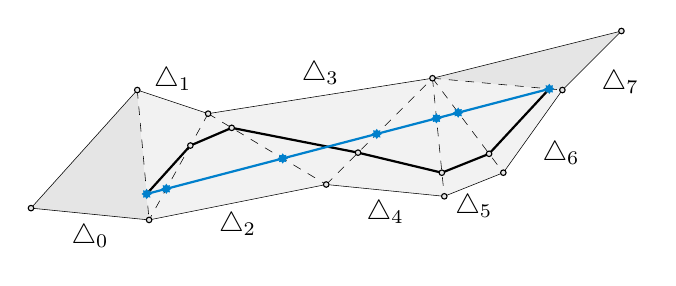
\begin{tikzpicture}[%
  >={Stealth[scale=1.0]},
  face/.style={star, star points = 8},
  scale=1.5,
]

  \tkzDefPoint(0.0, 0.0){v0}
  \tkzDefPoint(1.0, -0.1){v1}
  \tkzDefPoint(0.9, 1.0){v2}
  \tkzDefPoint(1.5, 0.8){v3}
  \tkzDefPoint(2.5, 0.2){v4}
  \tkzDefPoint(3.4, 1.1){v5}
  \tkzDefPoint(3.5, 0.1){v6}
  \tkzDefPoint(4.0, 0.3){v7}
  \tkzDefPoint(4.5, 1.0){v8}
  \tkzDefPoint(5.0, 1.5){v9}

  \tkzDefPointOnLine[pos=0.2](v1,v2)\tkzGetPoint{e0}
  \tkzDefPointOnLine[pos=0.7](v1,v3)\tkzGetPoint{e1}
  \tkzDefPointOnLine[pos=0.2](v3,v4)\tkzGetPoint{e2}
  \tkzDefPointOnLine[pos=0.3](v4,v5)\tkzGetPoint{e3}
  \tkzDefPointOnLine[pos=0.8](v5,v6)\tkzGetPoint{e4}
  \tkzDefPointOnLine[pos=0.8](v5,v7)\tkzGetPoint{e5}
  \tkzDefPointOnLine[pos=0.9](v5,v8)\tkzGetPoint{e6}

  \tkzInterLL(e0,e6)(v1,v2)\tkzGetPoint{g0}
  \tkzInterLL(e0,e6)(v1,v3)\tkzGetPoint{g1}
  \tkzInterLL(e0,e6)(v3,v4)\tkzGetPoint{g2}
  \tkzInterLL(e0,e6)(v4,v5)\tkzGetPoint{g3}
  \tkzInterLL(e0,e6)(v5,v6)\tkzGetPoint{g4}
  \tkzInterLL(e0,e6)(v5,v7)\tkzGetPoint{g5}
  \tkzInterLL(e0,e6)(v5,v8)\tkzGetPoint{g6}

  \tkzFillPolygon[color=black!10](v0,v1,v2)
  \tkzFillPolygon[color=black!5](v3,v1,v2)
  \tkzFillPolygon[color=black!5](v3,v1,v4)
  \tkzFillPolygon[color=black!5](v3,v5,v4)
  \tkzFillPolygon[color=black!5](v6,v5,v4)
  \tkzFillPolygon[color=black!5](v6,v5,v7)
  \tkzFillPolygon[color=black!5](v8,v5,v7)
  \tkzFillPolygon[color=black!10](v8,v5,v9)

  \tkzDrawSegments[dashed](v2,v1 v3,v1 v3,v4 v4,v5 v5,v6 v5,v7 v5,v8)
  \tkzDrawSegments(v0,v1 v0,v2 v2,v3 v1,v4 v3,v5 v4,v6 v6,v7 v7,v8 v8,v9 v5,v9)
  \tkzDrawPoints(v0,v1,v2,v3,v4,v5,v6,v7,v8,v9)

  \tkzDrawSegments[thick](e0,e1 e1,e2 e2,e3 e3,e4 e4,e5 e5,e6)
  \tkzDrawPoints(e0,e1,e2,e3,e4,e5,e6)

  \tkzDrawSegments[thick,myblue](g0,g1 g1,g2 g2,g3 g3,g4 g4,g5 g5,g6)
  \tkzDrawPoints[star,star points=8,myblue,scale=1.5](g0,g1,g2,g3,g4,g5,g6)

  \tkzLabelSegment[below](v0,v1){$\triangle_0$}
  \tkzLabelSegment[above](v2,v3){$\triangle_1$}
  \tkzLabelSegment[below](v1,v4){$\triangle_2$}
  \tkzLabelSegment[above](v3,v5){$\triangle_3$}
  \tkzLabelSegment[below](v4,v6){$\triangle_4$}
  \tkzLabelSegment[below](v6,v7){$\triangle_5$}
  \tkzLabelSegment[below right](v7,v8){$\triangle_6$}
  \tkzLabelSegment[below right](v8,v9){$\triangle_7$}

\end{tikzpicture}
\end{document}
